\documentclass{bioinfo}
\copyrightyear{2016} \pubyear{2016}

%% Some pieces required from the pandoc template
\providecommand{\tightlist}{%
  \setlength{\itemsep}{0pt}\setlength{\parskip}{0pt}}


% Pandoc citation processing


% hyperref makes the margins screwy.
% https://groups.google.com/forum/#!topic/latexusersgroup/4W_SwGk6zx4
% http://ansuz.sooke.bc.ca/software/latex-tricks.php
% \usepackage[colorlinks=true, allcolors=blue]{hyperref}

\access{Advance Access Publication Date:   }
\appnotes{Manuscript Category}

\begin{document}
\firstpage{1}

\subtitle{Application Note}

\title[JBrowseR: R Interface to JBrowse 2]{JBrowseR: An R Interface to
the JBrowse 2 Genome Browser}

\author[FirstAuthorLastName \textit{et~al}.]{
Elliot Hershberg\,\textsuperscript{1},
Garrett Stevens\,\textsuperscript{1},
Colin Diesh\,\textsuperscript{1},
Peter Xie\,\textsuperscript{1},
Teresa De Jesus Martinez\,\textsuperscript{1},
Rob Buels\,\textsuperscript{1},
Lincoln Stein\,\textsuperscript{2},
Ian Holmes\,\textsuperscript{1*},
}

\address{
\textsuperscript{1}Department of Bioengineering, University of
California, Berkeley, Berkeley, CA 94720, USA\\
\textsuperscript{2}Ontario Institute for Cancer Research, Toronto, ON
M5G 0A3, Canada\\
}

\corresp{*To whom correspondence should be addressed. E-mail:
ihh@berkeley.edu}

\history{Received on XXX; revised on XXX; accepted on XXX}

\editor{Associate Editor: XXX}

\abstract{
\textbf{Motivation:} Genome browsers are an essential tool in genome
analysis. Modern genome browsers enable complex and interactive
visualization of a wide variety of genomic data modalities. While such
browsers are very powerful, they can be challenging to configure and
program for bioinformaticians lacking expertise in web development.\\
\textbf{Results:} We have developed an R package that provides an
interface to the JBrowse 2 genome browser. The package can be used to
configure and customize the browser entirely with R code. The browser
can be deployed from the R console, or embedded in Shiny applications or
R Markdown documents.\\
\textbf{Availability:} JBrowseR is available for download from CRAN, and
the source code is openly available from the Github repository at
\href{https://github.com/GMOD/JBrowseR/}{https://github.com/GMOD/JBrowseR/}.\\
\textbf{Contact:}ihh@berkeley.edu\\
\textbf{Supplementary information:} Supplementary data are available at
Bioinformatics Online.}

\maketitle

\section{Introduction}

The development of genome browsers has been described as a milestone of
the genomic revolution \citep{packer2007clickable}. Genome browsers
provide researchers with the ability to visualize and explore genomic
annotations and data. Due to their widespread adoption and use, the
linear display of genomic information along reference coordinates is one
of the most common representations of biological data in the 21st
century.

Since their original development during the advent of genome sequencing
\citep{kent2002human, birney2004overview}, genome browsers have made
considerable gains in performance and sophistication. One important
development has been the implementation of genome browsers in
JavaScript, beginning with JBrowse \citep{buels2016jbrowse}. Leveraging
JavaScript---along with modern web technologies such as Canvas and
SVG---makes it possible to move computation that previously took place
on a server into the client web browser, as well as offering a more
responsive and interactive experience to the user.

JBrowse 2 is an extensible platform for visualizing and integrating
biological data, consisting of a ground-up rewrite of JBrowse using
ReactJS and TypeScript. The platform can be configured and deployed with
custom data and settings, enabling research communities to develop and
maintain curated sets of resources and data on the web, such as WormBase
for the \emph{C. elegans} community \citep{harris2010wormbase}.

JBrowse 2 contains many new views and components, to be described in a
later paper. However, one core part is a React component that renders a
configurable linear genome browser, enabling researchers to embed custom
browsers into existing React applications. While the JBrowse 2 React
linear genome view component is powerful and extensible, its use can
present an obstacle to bioinformaticians who don't have experience with
React development. On the other hand, the R programming language and
environment is widely used in the bioinformatics community, as evidenced
by the size and and usage of efforts such as Bioconductor
\citep{huber2015orchestrating}.

To bridge this gap, we introduce JBrowseR, an R interface the JBrowse 2
genome browser. JBrowseR is an R package with functions for embedding a
custom browser instance in a Shiny app, R Markdown document, or the R
console.

\section{Materials and Methods}

JBrowseR is implemented as an R package and distributed on CRAN. The
package was built according to the R best practices encoded in the
devtools package, ensuring continual use of R CMD Check and maintaining
consistent and robust function documentation during development. The
core rendering methods of the library rely on the htmlwidgets framework,
which can be used to embed JavaScript visualization tools in R Shiny
apps, as well as R Markdown documents. Htmlwidgets can also can be used
from an R interactive console. Using the reactR package, JBrowseR
renders the JBrowse 2 widget inside of a root HTML element in an
htmlwidget.

The interface of JBrowseR enables users to generate JBrowse 2
configuration for their own data using simple R functions. The
configuration values can be composed together to create an arbitrarily
complex custom browser. The majority of genomic data formats commonly
displayed in genome browsers are supported, including (but not limited
to) FASTA, BED, GFF3, BAM, CRAM, VCF, Wiggle, and bigWig. JBrowseR also
includes an HTTP server for serving local data that is configured with
the necessary settings and features for working with genome browsers
such as JBrowse and IGV.js
\citep{robinson2011integrative, robinson2017variant}.

The source code for JBrowseR is hosted on GitHub, and is automatically
tested using continuous integration running on the Windows, MacOS and
Linux operating systems. Automated tests for the package are implemented
using the testthat R package.

\begin{figure}
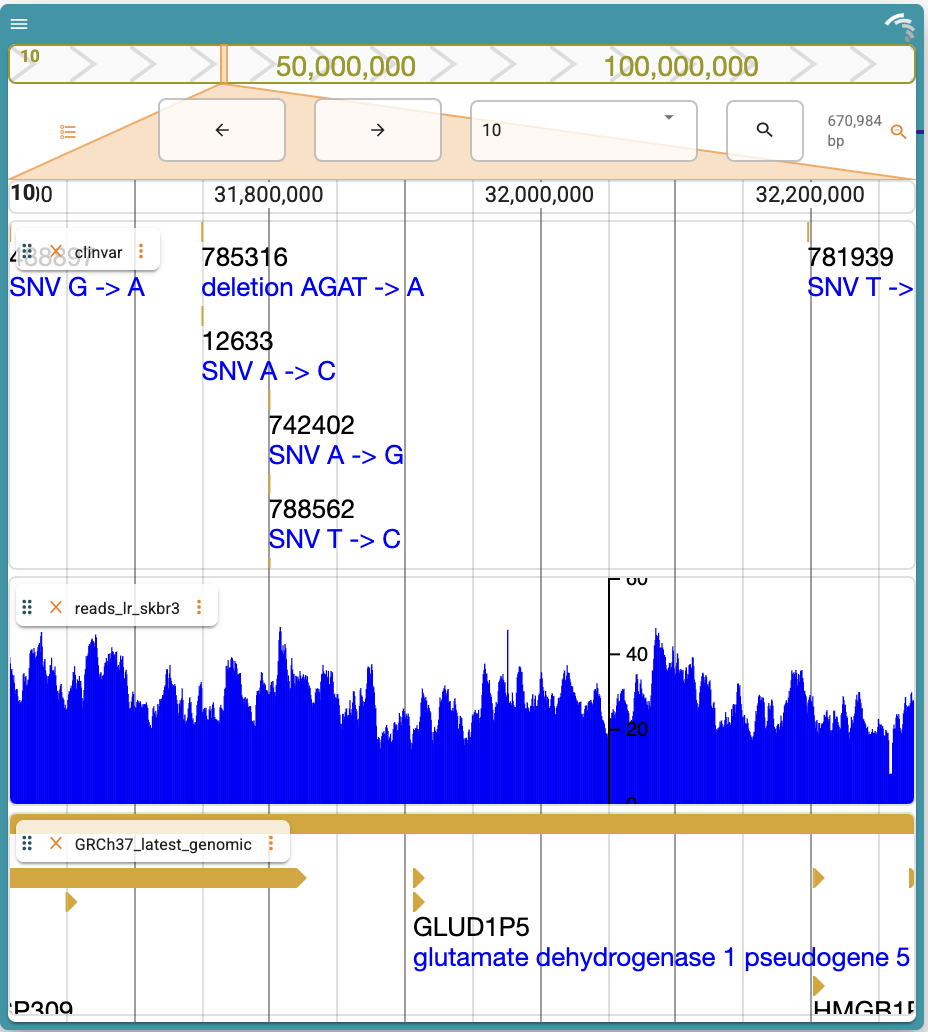
\includegraphics[width=1\linewidth]{JBrowseR-paper-fig1} \caption{A custom JBrowse 2 genome browser generated using JBrowseR.}\label{fig:unnamed-chunk-1}
\end{figure}

\section{Results and Discussion}

In order to demonstrate the utility of JBrowseR, several Shiny apps were
built and are included along with the package source code on GitHub. One
of the included apps demonstrates adding CRAM, VCF, GFF3, and bigWig
data (fig.~1), as well as setting a custom color palette for the
browser. Another one of the provided demo apps illustrates how JBrowseR
can also be configured with a JSON file (like other JBrowse 2 apps) by
loading the Sars-CoV-2 reference genome and NCBI annotations from a
JBrowse 2 configuration file. Finally, we have provided an example
deployment of JBrowseR in an app with interactions connected to other R
shiny UI components at
\href{https://elliothershberg.shinyapps.io/sars-cov-2-spike-mutations/}{https://elliothershberg.shinyapps.io/sars-cov-2-spike-mutations/}.

One of the core strengths of JBrowseR is its versatility. It
considerably lowers the level of expertise required to create a
web-facing genome database with a fast and flexible genome annotation
browser. However, web applications are not the only available target
point for the rendering functions: JBrowseR can also embed a genome
browser into R Markdown, a flexible documentation format that is used to
write scientific articles (including this one). We anticipate that as
platforms such as eLife's ``reproducible article''
\citep{maciocci2019introducing} mature and become more widely adopted,
it will be possible for genomics articles to contain interactive genome
browsers such as JBrowseR displaying their data.

\section{Availability}

JBrowseR is freely available for download from CRAN, and the source code
is publicly available at
\href{https://github.com/GMOD/JBrowseR/}{https://github.com/GMOD/JBrowseR/}.
The package reference guide and tutorials can be found at
\href{https://gmod.github.io/JBrowseR/}{https://gmod.github.io/JBrowseR/}.

\section*{Acknowledgements}
\addcontentsline{toc}{section}{Acknowledgements}

We thank the reactR authors Kent Russell and Alan Dipert for creating
and maintaining a clean interface between React and htmlwidgets, which
spurred the experiment into whether or not a package such as JBrowseR
would be feasible.

\section*{Funding}
\addcontentsline{toc}{section}{Funding}

This work was funded by NIH grants HG004483 and GM080203.


% Bibliography
\bibliographystyle{natbib}
\bibliography{bibliography.bib}

\end{document}
